\documentclass[10pt,aspectratio=169]{beamer}

\usetheme[progressbar=foot]{metropolis}
\AtBeginSection{}

\usepackage{appendixnumberbeamer}
\usepackage{booktabs}
\usepackage[scale=2]{ccicons}
\usepackage{tabularx}
\usepackage{tikz}
\usetikzlibrary{arrows.meta,positioning,shapes.geometric,fit}
\usepackage{xspace}
\newcommand{\themename}{\textbf{\textsc{metropolis}}\xspace}
\usepackage{comment}
\usepackage{caption}
\usepackage[
  backend=biber,
  style=authoryear
]{biblatex}

\setbeamertemplate{bibliography item}{}
\addbibresource{bibliography.bib}

\usepackage{graphicx}
\usepackage{siunitx}



%................................................................................
% COLORS

\definecolor{ukudlaBlue}{RGB}{41, 60, 135}
\definecolor{ukudlaLightBlue}{RGB}{212, 216, 231}
\definecolor{ukudlaRed}{RGB}{164, 28, 34}
\definecolor{ukudlaLightRed}{RGB}{236, 209, 210}
\definecolor{ukudlaGreen}{RGB}{59, 139, 71}
\definecolor{ukudlaLightGreen}{RGB}{215, 231, 218}
\definecolor{ukudlaYellow}{RGB}{239, 198, 44}
\definecolor{ukudlaLightYellow}{RGB}{251, 243, 212}
\definecolor{white}{RGB}{255, 255, 255}
\definecolor{black}{RGB}{0, 0, 0}

\setbeamercolor{palette primary}{fg=white, bg=ukudlaGreen}
\setbeamercolor{progress bar}{fg=ukudlaRed, bg=ukudlaYellow}
\setbeamercolor{title separator}{fg=ukudlaRed, bg=ukudlaYellow}
\setbeamercolor{progress bar in head/foot}{fg=ukudlaRed, bg=ukudlaYellow}
\setbeamercolor{progress bar in section page}{fg=ukudlaRed, bg=ukudlaYellow}
\setbeamercolor{background canvas}{bg=white}



%................................................................................
% PRESENTATION INFORMATION

\title{UKUDLA Data Science Certificate}
\subtitle{Remote Computing using SSH \& Linux}
\author{Markus Mößler}
\institute{University of Hohenheim}



%................................................................................
% CUSTOM FOOTER

\makeatletter
\setbeamertemplate{progress bar in head/foot}{%
  \tikzset{metropolis@progressbar@foreground/.style={fill=ukudlaGreen}}%
  \tikzset{metropolis@progressbar@background/.style={fill=ukudlaLightGreen}}%

  \begin{tikzpicture}[overlay, x=\paperwidth, y=1cm]
    \fill[metropolis@progressbar@background]
      (0,0) rectangle (1,0.10);
    \fill[metropolis@progressbar@foreground]
      (0,0) rectangle
      ({\insertframenumber/\inserttotalframenumber},0.10);
    \node[anchor=south west, yshift=0.25cm, xshift=0.2cm]
      at (0,0)
      {\includegraphics[height=0.75cm]{./logos/UKUDLA_logo_03_white_bg.pdf}};
    % current section
    \ifnum\value{section}>0
      \node[
        anchor=south east,
        yshift=0.22cm,
        xshift=-0.60cm,
        fill=ukudlaLightGreen,
        rounded corners=2pt,
        inner xsep=6pt,
        inner ysep=3pt,
        font=\scriptsize\bfseries,
        text=ukudlaRed
      ] at (1,0) {
        \insertsectionhead
      };
    \fi

  \end{tikzpicture}%
}
\makeatother



%................................................................................
% CUSTOM TITLE PAGE

\makeatletter
\setbeamertemplate{title page}{
  \begin{beamercolorbox}[sep=8pt, center, wd=\paperwidth, ht=0.5\paperheight]{title page top}
    \begin{minipage}[c]{1.00\textwidth}
      \raggedleft
      \includegraphics[height=1.00cm]{./logos/ukudla_universities.pdf}
      \vspace*{0.2cm}
    \end{minipage}
    \begin{beamercolorbox}[wd=0.9\paperwidth, sep=12pt, left]{top box}
      {\usebeamerfont{title}\usebeamercolor[fg]{title}\inserttitle\par}
      \vskip0.1cm
      {\usebeamerfont{subtitle}\usebeamercolor[fg]{subtitle}\insertsubtitle\par}
    \end{beamercolorbox}
  \end{beamercolorbox}
  \begin{beamercolorbox}[sep=8pt, center, wd=\paperwidth, ht=0.5\paperheight]{title page bottom}
    \begin{beamercolorbox}[wd=0.9\paperwidth, sep=12pt, left]{bottom box}
      \hbox{%
        \hspace*{1em}
        \begin{minipage}[c]{0.40\textwidth}
          \vskip1.0cm
          {\usebeamerfont{author}\usebeamercolor[fg]{author}\insertauthor\par}
          \vskip0.1cm
          {\usebeamerfont{institute}\usebeamercolor[fg]{institute}\insertinstitute\par}
        \end{minipage}%
        \hspace*{1.5cm}
        \begin{minipage}[c]{1.00\textwidth}
          \includegraphics[height=2.0cm]{./logos/UKUDLA_logo_05.pdf}
        \end{minipage}%
      }
    \end{beamercolorbox}
    \begin{minipage}[r]{1.00\textwidth}
      \centering
      \includegraphics[width=1.00\textwidth]{./logos/ukudla_sponsors.pdf}
    \end{minipage}
  \end{beamercolorbox}
}
\makeatother

\setbeamercolor{title page top}{bg=white}
\setbeamercolor{top box}{bg=ukudlaGreen}
\setbeamercolor{title page bottom}{bg=white}
\setbeamercolor{bottom box}{bg=ukudlaLightGreen}
\setbeamercolor{title}{fg=white}
\setbeamercolor{subtitle}{fg=white}
\setbeamercolor{author}{fg=black}
\setbeamercolor{institute}{fg=black}
\setbeamercolor{date}{fg=black}

\setbeamercolor{block body}{bg=ukudlaLightGreen,fg=black}



%................................................................................
% DOCUMENT

\begin{document}

\maketitle

%--------------------------------------------------
{
\setbeamertemplate{frame numbering}[none]

\begin{frame}[noframenumbering]{Table of contents}

  \small
  \setbeamertemplate{section in toc}[sections numbered]
  \tableofcontents[hideallsubsections]

\end{frame}
}
%--------------------------------------------------



\section{Motivation}


%--------------------------------------------------
% CONTENT SLIDE 1/10
\begin{frame}{One project in different computing contexts}

\small

\centering

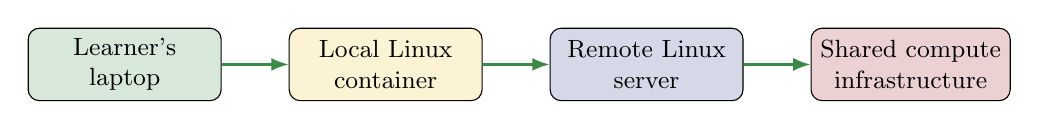
\begin{tikzpicture}[
  box/.style={
    draw,
    rounded corners,
    minimum width=2.45cm,
    minimum height=0.92cm,
    align=center,
    font=\small
  },
  arrow/.style={-{Latex[length=2.2mm]},thick,ukudlaGreen}
]
  \node[box,fill=ukudlaLightGreen] (laptop) {Learner's\\laptop};
  \node[box,fill=ukudlaLightYellow,right=0.85cm of laptop] (container)
    {Local Linux\\container};
  \node[box,fill=ukudlaLightBlue,right=0.85cm of container] (server)
    {Remote Linux\\server};
  \node[box,fill=ukudlaLightRed,right=0.85cm of server] (cluster)
    {Shared compute\\infrastructure};
  \draw[arrow] (laptop) -- (container);
  \draw[arrow] (container) -- (server);
  \draw[arrow] (server) -- (cluster);
\end{tikzpicture}

\vspace{0.50cm}

\begin{columns}[T]

\column{0.31\textwidth}
\textbf{Linux}
\begin{itemize}
  \item Operating-system family
  \item Common on servers and containers
\end{itemize}

\column{0.31\textwidth}
\textbf{Terminal}
\begin{itemize}
  \item Text-based interface
  \item Displays input and output
\end{itemize}

\column{0.33\textwidth}
\textbf{Shell}
\begin{itemize}
  \item Reads and runs commands
  \item Bash is a common shell
\end{itemize}

\end{columns}

\end{frame}
%--------------------------------------------------


%--------------------------------------------------
% CONTENT SLIDE 2/10
\begin{frame}{Why the command line matters in data science}

\small

\begin{columns}[T]

\column{0.50\textwidth}

\textbf{Repeatable work}

\begin{itemize}
  \item Commands can be saved in scripts.
  \item The same instruction can process many files.
  \item Text commands are easy to document and review.
\end{itemize}

\column{0.47\textwidth}

\textbf{Portable work}

\begin{itemize}
  \item Remote systems may have no desktop.
  \item Small tools can be combined.
  \item Automation scales beyond manual clicking.
\end{itemize}

\end{columns}

\vspace{0.50cm}

\begin{beamercolorbox}[rounded=true,sep=8pt]{block body}
The command line is not only a different interface. It expresses repeatable operations in a form that computers and collaborators can execute.
\end{beamercolorbox}

\end{frame}
%--------------------------------------------------



\section{Concepts}


%--------------------------------------------------
% CONTENT SLIDE 3/10
\begin{frame}{SSH: one secure connection, different outcomes}

\small

\centering

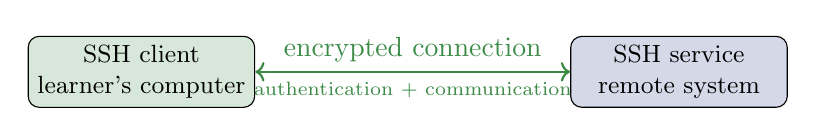
\begin{tikzpicture}[
  box/.style={
    draw,
    rounded corners,
    minimum width=2.75cm,
    minimum height=0.90cm,
    align=center,
    font=\small
  },
  arrow/.style={<->,thick,ukudlaGreen}
]
  \node[box,fill=ukudlaLightGreen] (client)
    {SSH client\\learner's computer};
  \node[box,fill=ukudlaLightBlue,right=4.0cm of client] (server)
    {SSH service\\remote system};
  \draw[arrow] (client) --
    node[above]{encrypted connection}
    node[below,font=\scriptsize]{authentication + communication}
    (server);
\end{tikzpicture}

\vspace{0.50cm}

\begin{columns}[T]

\column{0.47\textwidth}

\textbf{GitHub repository access}

\begin{itemize}
  \item Clone, fetch, pull, and push
  \item Exchange Git objects
  \item No general-purpose shell
\end{itemize}

\column{0.47\textwidth}

\textbf{Remote computing}

\begin{itemize}
  \item Open a remote shell
  \item Run programs and manage files
  \item Transfer files securely
\end{itemize}

\end{columns}

\end{frame}
%--------------------------------------------------


%--------------------------------------------------
% CONTENT SLIDE 4/10
\begin{frame}{Public-key authentication}

\small

\centering


\begin{tikzpicture}[
  key/.style={
    draw,
    rounded corners,
    minimum width=3.1cm,
    minimum height=1.2cm,
    align=center
  },
  arrow/.style={-{Latex[length=2.3mm]},thick,ukudlaGreen}
]
  \node[key,fill=ukudlaLightRed] (private)
    {Private key\\stays with the learner};
  \node[key,fill=ukudlaLightGreen,right=4.2cm of private] (public)
    {Public key\\registered with a service};
  \draw[arrow] (private) --
    node[above]{cryptographic proof}
    node[below,font=\scriptsize]{private key is not transmitted}
    (public);
\end{tikzpicture}

\vspace{0.50cm}

\raggedright

\begin{itemize}
  \item The public key may be shared; the private key must remain private.
  \item A passphrase protects the private key if its file is exposed.
  \item The server checks that the client controls the matching private key.
  \item Host fingerprints help verify that the client reached the intended host.
\end{itemize}

\end{frame}
%--------------------------------------------------


%--------------------------------------------------
% CONTENT SLIDE 5/10
\begin{frame}{A remote session changes the computing context}

\small

\centering

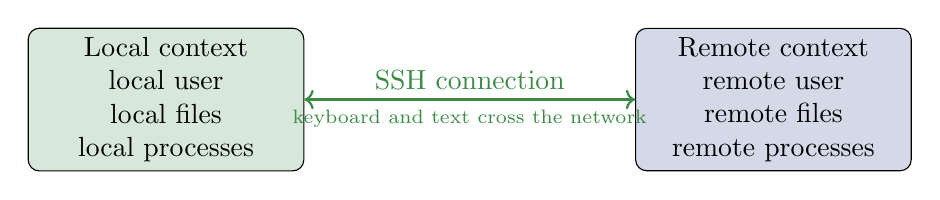
\begin{tikzpicture}[
  state/.style={
    draw,
    rounded corners,
    minimum width=3.5cm,
    minimum height=1.75cm,
    align=center
  },
  arrow/.style={<->,thick,ukudlaGreen}
]
  \node[state,fill=ukudlaLightGreen] (local)
    {Local context\\local user\\local files\\local processes};
  \node[state,fill=ukudlaLightBlue,right=4.2cm of local] (remote)
    {Remote context\\remote user\\remote files\\remote processes};
  \draw[arrow] (local) --
    node[above]{SSH connection}
    node[below,font=\scriptsize]{keyboard and text cross the network}
    (remote);
\end{tikzpicture}

\vspace{0.50cm}

\raggedright

Always establish context before acting:

\begin{itemize}
  \item Which computer and user am I controlling?
  \item Which directory and repository am I in?
  \item Which files and processes will this command affect?
\end{itemize}

\end{frame}
%--------------------------------------------------



%--------------------------------------------------
% CONTENT SLIDE 6/10
\begin{frame}[fragile]{Navigate and combine small Linux tools}

\scriptsize

\begin{columns}[T]

\column{0.38\textwidth}

\begin{verbatim}
/
|-- home/
|   `-- student/
|       `-- analysis-project/
|-- tmp/
`-- work/
\end{verbatim}

\column{0.58\textwidth}

\small

\begin{verbatim}
head results/summary.csv |
  column -s, -t
\end{verbatim}

\textbf{Navigation and composition}

\begin{itemize}
  \item Absolute paths begin at \texttt{/}.
  \item Relative paths begin at the current directory.
  \item A pipe connects one command's output to the next.
\end{itemize}

\end{columns}

\vspace{0.25cm}

\begin{beamercolorbox}[rounded=true,sep=8pt]{block body}
Commands operate in a context. Confirm the current directory before reading, writing, moving, or deleting files.
\end{beamercolorbox}

\end{frame}
%--------------------------------------------------


%--------------------------------------------------
\section{Application}
% CONTENT SLIDE 7/10

\begin{frame}{A container is a safe Linux practice environment}

\small

\centering

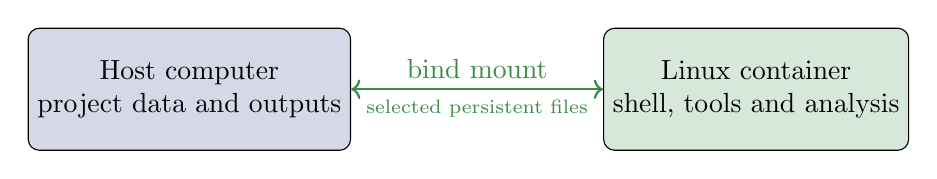
\begin{tikzpicture}[
  box/.style={
    draw,
    rounded corners,
    minimum width=3.2cm,
    minimum height=1.55cm,
    align=center
  },
  arrow/.style={<->,thick,ukudlaGreen}
]
  \node[box,fill=ukudlaLightBlue] (host)
    {Host computer\\project data and outputs};
  \node[box,fill=ukudlaLightGreen,right=3.2cm of host] (container)
    {Linux container\\shell, tools and analysis};
  \draw[arrow] (host) --
    node[above]{bind mount}
    node[below,font=\scriptsize]{selected persistent files}
    (container);
\end{tikzpicture}

\vspace{0.50cm}

\raggedright

\begin{itemize}
  \item The image supplies a consistent Linux environment.
  \item A temporary container can be explored and discarded.
  \item Source copied into the image is a build-time snapshot.
  \item Bind-mounted inputs and outputs remain on the host.
\end{itemize}

\end{frame}
%--------------------------------------------------



%--------------------------------------------------
% CONTENT SLIDE 8/10
\begin{frame}{One data science project across several contexts}

\centering

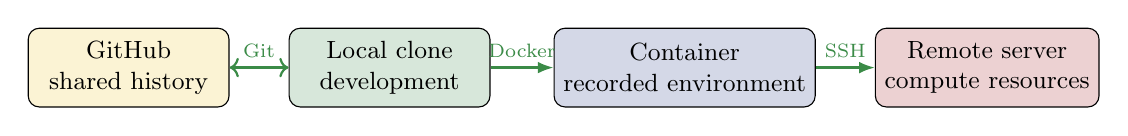
\begin{tikzpicture}[
  context/.style={
    draw,
    rounded corners,
    minimum width=2.55cm,
    minimum height=1.0cm,
    align=center,
    font=\small
  },
  arrow/.style={-{Latex[length=2mm]},thick,ukudlaGreen}
]
  \node[context,fill=ukudlaLightYellow] (git)
    {GitHub\\shared history};
  \node[context,fill=ukudlaLightGreen,right=0.75cm of git] (local)
    {Local clone\\development};
  \node[context,fill=ukudlaLightBlue,right=0.80cm of local] (container)
    {Container\\recorded environment};
  \node[context,fill=ukudlaLightRed,right=0.75cm of container] (remote)
    {Remote server\\compute resources};

  \draw[arrow,<->] (git) -- node[above,font=\scriptsize]{Git} (local);
  \draw[arrow] (local) -- node[above,font=\scriptsize]{Docker} (container);
  \draw[arrow] (container) -- node[above,font=\scriptsize]{SSH} (remote);
\end{tikzpicture}

\vspace{0.50cm}

\small

\begin{itemize}
  \item Git identifies and exchanges project states.
  \item Docker describes and builds the execution environment.
  \item SSH provides secure access to another computer.
  \item Linux commands operate the project in containers and on servers.
\end{itemize}

\end{frame}
%--------------------------------------------------



%--------------------------------------------------
% CONTENT SLIDE 9/10
\begin{frame}{Command-line and remote-computing care}

\small

\begin{columns}[T]

\column{0.48\textwidth}

\textbf{Before a command}

\begin{itemize}
  \item Confirm the host and user.
  \item Confirm the current directory.
  \item Inspect targets and command options.
  \item Understand persistence and permissions.
\end{itemize}

\column{0.48\textwidth}

\textbf{For shared infrastructure}

\begin{itemize}
  \item Protect credentials and private keys.
  \item Respect CPU, memory, and storage limits.
  \item Manage long-running work appropriately.
  \item Preserve outputs and stop unneeded processes.
\end{itemize}

\end{columns}

\vspace{0.25cm}

\begin{beamercolorbox}[rounded=true,sep=8pt]{block body}
SSH secures the connection. It does not make every command safe, every server trusted, or every analysis scientifically correct.
\end{beamercolorbox}

\end{frame}
%--------------------------------------------------


%--------------------------------------------------
\section{Key Message}
% CONTENT SLIDE 10/10

\begin{frame}{Key message: know which computer a command affects}

\large

\begin{enumerate}
  \item Linux, a terminal, a shell, and SSH are related but distinct.
  \item SSH authenticates and protects communication with a remote service.
  \item A remote shell operates another computer, not the local laptop.
  \item Linux commands provide a repeatable interface across containers and
        servers.
  \item Git, Docker, SSH, and Linux connect one data science project across
        several computing contexts.
\end{enumerate}

\vspace{0.25cm}

\small
\centering
Detailed commands, exercises, verification, and troubleshooting are provided in the learning-module guides.

\end{frame}
%--------------------------------------------------


%--------------------------------------------------
\begin{frame}[plain,noframenumbering]{Supported by}

  South African government and the National Research Foundation

  \begin{flushleft}
    \includegraphics[trim=0cm 0cm 0cm 0cm, clip, width=0.50\textwidth]{./logos/ukudla_south_african_sponsors.pdf}
  \end{flushleft}

  German government and the German Academic Exchange Service

  \begin{flushleft}
    \includegraphics[trim=0cm 0cm 0cm 0cm, clip, width=1.00\textwidth]{./logos/ukudla_german_sponsors.pdf}
  \end{flushleft}

\end{frame}
%--------------------------------------------------

\end{document}
